\documentclass[11pt,a4paper]{article}
\usepackage[margin=0.82in]{geometry}
\usepackage{amsmath,amssymb,amsfonts}
\usepackage{booktabs}
\usepackage{graphicx}
\usepackage{xcolor}
\usepackage{hyperref}
\usepackage{multirow}
\usepackage{caption}

\hypersetup{
    colorlinks=true,
    linkcolor=blue!70!black,
    citecolor=blue!70!black,
    urlcolor=blue!70!black
}

\title{\textbf{An AI Agent's Weight-Space Anatomy and Zero-Training LoRA Surgery:\\Autonomous Discovery and Repair of Middle-Layer Relational Circuits vs.\ Late-Layer Readout Valves}}
\author{
  \textbf{Tao Li}$^{1}$ \quad
  \textbf{Junfeng Liu}$^{2,*}$ \quad
  \textbf{Qiang Shen}$^{3}$ \quad
  \textbf{Bo Shao}$^{3}$ \quad
  \textbf{Linjun Shou}$^{3}$ \quad
  \textbf{Xuejun Liu}$^{1}$ \\[4pt]
  $^{1}$Nanjing University of Aeronautics and Astronautics \quad
  $^{2}$Pengcheng Laboratory \quad
  $^{3}$Microsoft \\[2pt]
  \texttt{litao037@nuaa.edu.cn}, \; \texttt{liujf@pcl.ac.cn}, \; \texttt{\{qiangshen, boshao, lisho\}@microsoft.com}, \; \texttt{xuejun.liu@nuaa.edu.cn} \\[2pt]
  {\small $^{*}$Corresponding author: Junfeng Liu (\texttt{liujf@pcl.ac.cn})}
}
\date{November 4, 2026}

\begin{document}
\maketitle

\begin{abstract}
Can an AI research agent autonomously diagnose why a fine-tuned language model fails on structured tasks—not by trial-and-error prompt engineering or hyperparameter sweeps, but by directly reading the model's weight matrices, localizing the defective sub-circuits, and editing the weights in closed form with zero gradient steps? Extending the paradigm of \emph{Weight-Space Programming} (Takehi et al., 2026) from toy single-model probes to 32-layer Low-Rank Adaptation (LoRA) post-training, we present an autonomous \textbf{Agentic Weight-Space Anatomy \& Zero-Training Surgery} loop. When investigating why standard Supervised Fine-Tuning (SFT) plateaus early or degrades with extended training (\emph{the Step-Count Paradox}) and why off-policy SFT and on-policy distillation (OPD / OPSD) exhibit opposite Precision--Recall trade-offs, the agent formulates and executes a three-step mathematical microscope on 21.2M-parameter LoRA tensors: (1) \textbf{Gauge-Invariant Reduced QR-SVD} to canonicalize low-rank $(A,B)$ displacements without forming dense $d_{\text{out}} \times d_{\text{in}}$ matrices; (2) \textbf{32-Layer $\times$ 6-Organ Subspace Alignment Scanning} across attention and FFN projections; and (3) \textbf{RMSNorm-Weighted Unembedding Vocabulary Projection} to decode which exact tokens each layer's leading singular vector $u_1$ promotes or suppresses.

Applying this autonomous anatomy across \textbf{four benchmarks}—three public NLP benchmarks (\textbf{Re-DocRED}, \textbf{BioRED}, \textbf{PHEE}) and a real-world industrial deployment (\textbf{Browser TabGroup})—as well as across model scales (\texttt{Qwen3.5-2B/4B/9B}) and architectures (\texttt{Ministral-3-8B}), the agent uncovers a universal phase transition at \textbf{Layer 18}: \textbf{middle layers} (\textbf{L06--L15}) form a shared cross-entity relational and fine-grained clustering circuit ($\cos(\Delta W_{\text{OPSD}}, \Delta W_{\text{SFT}})$ up to $0.37$), whereas \textbf{late layers} (\textbf{L18--L31}) act as a formatting and stopping \emph{readout valve} that diverges to orthogonality ($\cos \approx 0.00$) and concentrates SFT's surface/abstention overfitting ($8\times$--$78\times$ stronger projection onto \texttt{' \&'}, \texttt{Unrelated}, and \texttt{Ungrouped}). Guided by its own diagnostic map, the agent synthesizes \textbf{Zero-Training LoRA Surgeries} that require zero gradient steps: (i) \emph{Single-Model Valve \& Spectral Surgery} (\textbf{Idea A/B/C}) reverses SFT over-training degradation and boosts single-stage accuracy by $+6.38\text{pp}$ F1 on \texttt{Qwen3.5-2B}, $+4.28\text{pp}$ on \texttt{Qwen3.5-4B}, and $+2.44\text{pp}$ on \texttt{Ministral-3-8B} ($41.46\%$ F1 on \texttt{BioRED}; $+2.12\text{pp}$ Recall and $80.46\%$ F1 on \texttt{TabGroup}), while rescuing adapted SFT on \texttt{Re-DocRED} from $14.14\%$ to \textbf{$38.77\%$ F1}; and (ii) \emph{Dual-Adapter Circuit Grafting \& Spectral Consensus} (\textbf{\texttt{Graft-18}} and \textbf{\texttt{SVD-Blend-50/50}}) strictly dominate SFT, OPSD, and $9\text{B}\to 4\text{B}$ white-box OPD across all four benchmarks (\textbf{$35.95\%$ F1} on \texttt{BioRED}, \textbf{$91.18\%$ F1} on \texttt{PHEE}, and \textbf{$68.18\%$ F1 / $72.41\%$ Precision} on \texttt{Browser TabGroup}).
\end{abstract}

\section{Introduction}
A central aspiration of AI-driven scientific discovery is to move beyond treating neural networks as black boxes tuned via blind hyperparameter sweeps. Recently, Takehi et al. (2026) introduced \emph{Sparks of Weight-Space Programming}, demonstrating that a frontier LLM agent equipped with a Python execution environment can directly inspect the weights of a 0.8B parameter model and ablate 64 looping MLP neurons without gradient descent. However, a fundamental question remains open: \emph{Can an AI research agent scale weight-space introspection to modern 2B--9B post-trained language models, autonomously uncover universal mechanistic laws governing Supervised Fine-Tuning (SFT) versus On-Policy Distillation (OPD / OPSD), and design closed-form weight surgeries that outperform gradient-based post-training across diverse public and industrial benchmarks?}

In this paper, the AI research agent serves as the primary investigator—designing and executing an end-to-end \textbf{Weight-Space Anatomy $\to$ Mechanistic Law Discovery $\to$ Zero-Training LoRA Surgery} workflow on structured extraction (\texttt{Re-DocRED}, \texttt{BioRED}, \texttt{PHEE}) and real-world multi-tab browser organization (\texttt{Browser TabGroup}). Rather than assuming any manual two-stage training pipeline, the agent investigates why standard single-adapter LoRA SFT suffers from a pervasive \textbf{Step-Count Paradox} (where training longer degrades test F1) and why off-policy SFT and on-policy distillation exhibit opposite Precision--Recall trade-offs. By writing programmatic weight probes, the agent discovers that every single autoregressive forward pass on these tasks requires two distinct computations that collide under token-level cross-entropy:
\begin{enumerate}
    \item \textbf{Middle-Layer Relational \& Clustering Circuit (L06--L15):} Resolving multi-hop relationships across 15--35 entities or browser tabs and separating co-occurring sub-tasks or hierarchical argument roles (e.g., splitting \texttt{Treatment.Drug}, \texttt{Treatment.Dosage}, and \texttt{Treatment.Route} in \texttt{PHEE}, or separating fine-grained user intents in \texttt{TabGroup}).
    \item \textbf{Late-Layer Readout Formatting \& Stopping Valve (L18--L31):} Translating internal relational states into a strict output schema while calibrating the continuation-versus-termination boundary—deciding whether to emit a delimiter (\texttt{\textbackslash n} or \texttt{,}) to output another valid item or to emit an abstention/stopping marker (\texttt{Unrelated}, \texttt{Unassigned}, or \texttt{Ungrouped}).
\end{enumerate}

Through its three-stage weight-space anatomy protocol (Section~3), the agent proves that off-policy SFT continues to strengthen middle-layer relational representations as step count increases, but rapidly over-amplifies the top-1 singular mode ($\sigma_1$) in late readout layers—memorizing surface formatting tokens and overly conservative stopping thresholds that lock the readout valve. Directly inverting this diagnosis, the agent derives five zero-training surgical operators (\textbf{Idea A}, \textbf{Idea B-1/B-2}, \textbf{Idea C}, \textbf{\texttt{Graft-18}}, and \textbf{\texttt{SVD-Blend-50/50}}) and validates them across four benchmarks and four model architectures (\texttt{Qwen3.5-2B}, \texttt{Qwen3.5-4B}, \texttt{Qwen3.5-9B}, and 34-layer pure full-attention \texttt{Ministral-3-8B}).

\section{Related Work}
\paragraph{Structured Information Extraction \& LoRA Readout Bottlenecks.} Document-level relation extraction benchmarks such as \texttt{DocRED} (Yao et al., 2019), \texttt{Re-DocRED} (Tan et al., 2022), and \texttt{BioRED} (Luo et al., 2022), alongside hierarchical event extraction in \texttt{PHEE} (Sun et al., 2022), exhibit severe candidate-space imbalance ($>90\%$ \texttt{NA} pairs). Recent LLM-based DocRE studies report that direct LoRA fine-tuning yields high precision but low recall due to \texttt{NA} over-rejection, often forcing practitioners to train separate identification and extraction adapters at double inference cost.
\paragraph{On-Policy Distillation \& Weight-Space Programming.} Generalized Knowledge Distillation (GKD; Agarwal et al., 2024) and Self-Distilled Reasoner (OPSD; Zhao et al., 2026) supervise student rollouts using privileged teacher contexts. Concurrently, Takehi et al. (2026) introduced \emph{Weight-Space Programming}, showing that mechanistic weight edits can unlock latent model capabilities by removing output obstacles, while noting that weight edits alone cannot instill missing distributed representations. We unify these perspectives across three public extraction benchmarks and industrial browser session grouping via exact low-rank QR-SVD anatomy.

\section{How the AI Agent Anatomizes LoRA Weight Space: A Three-Step Methodology}

\subsection{Step 1: Gauge-Invariant Reduced QR-SVD of Low-Rank Displacements}
Unlike raw base weights, a LoRA adapter stores updates in factored form $\Delta W_m = s B_m A_m$ ($A_m \in \mathbb{R}^{r \times d_{\text{in}}}, B_m \in \mathbb{R}^{d_{\text{out}} \times r}, r=16, s=\alpha/r=2.0$), which suffers from \emph{gauge ambiguity}: for any invertible matrix $R \in \mathbb{R}^{r \times r}$, $(B_m R)(R^{-1} A_m) = B_m A_m$, meaning raw parameter vectors cannot be compared directly across checkpoints. Furthermore, materializing all 248 dense $d_{\text{out}} \times d_{\text{in}}$ matrices ($9216 \times 2560$) for full SVD is computationally wasteful. To inspect weight space rapidly and exactly, the agent formulates a \textbf{Gauge-Invariant Reduced QR-SVD} algorithm that operates in $<0.5$ seconds per checkpoint:
\begin{enumerate}
    \item For a single adapter $\Delta W_m = s B_m A_m$ (or the relative displacement $\Delta W_m = s(B_{1,m} A_{1,m} - B_{0,m} A_{0,m}) = s [B_{1,m}, -B_{0,m}] [A_{1,m}^\top, A_{0,m}^\top]^\top$ from a reference checkpoint $W_0$), compute thin QR factorizations $Q_B R_B = \text{LeftFactor}$ and $Q_A R_A = \text{RightFactor}^\top$, where $R_B, R_A \in \mathbb{R}^{k \times k}$ ($k \in \{16, 32\}$).
    \item Compute the SVD of the tiny $k \times k$ core matrix $R_B R_A^\top = \tilde{U} \Sigma \tilde{V}^\top$, where $\Sigma = \operatorname{diag}(\sigma_1, \dots, \sigma_k)$ with $\sigma_1 \ge \dots \ge \sigma_k$.
    \item Recover the exact orthonormal left (output-space) singular vectors $U = Q_B \tilde{U} \in \mathbb{R}^{d_{\text{out}} \times k}$ and right (input-space) singular vectors $V = Q_A \tilde{V} \in \mathbb{R}^{d_{\text{in}} \times k}$.
\end{enumerate}

\subsection{Step 2: 32-Layer $\times$ 6-Organ Functional Cartography}
We conduct our primary anatomy on \texttt{Qwen/Qwen3.5-4B} (32 layers: 24 Gated-DeltaNet linear-attention layers interleaved with 8 full-attention layers at $L \in \{3,7,11,15,19,23,27,31\}$; $d_{\text{model}}=2560, d_{\text{ff}}=9216$), and further verify cross-scale and cross-architecture generalization on \texttt{Qwen/Qwen3.5-2B} (24L), \texttt{Qwen/Qwen3.5-9B} (32L), and \texttt{mistralai/Ministral-3-8B-Instruct} (34L pure full-attention Transformer) in Section~5. The agent maps each Transformer layer into 6 physical sub-modules (the 6 rows of Figure~\ref{fig:heatmap}A):
\begin{enumerate}
    \item \textbf{\texttt{MLP GateProj} ($2560 \to 9216$):} Non-linear SiLU switch $\sigma(W_{\text{gate}} h)$ gating which FFN neurons fire.
    \item \textbf{\texttt{MLP UpProj} ($2560 \to 9216$):} Semantic feature extractor multiplied elementwise with the gate.
    \item \textbf{\texttt{MLP DownProj} ($9216 \to 2560$, Residual Writer):} Projects active FFN neurons back to the residual stream; each column $j \in \{1,\dots,9216\}$ acts as an atomic vocabulary valve pushing continuation tokens (\texttt{\textbackslash n}, \texttt{,}) vs.\ termination tokens (\texttt{Unrelated}, \texttt{Unassigned}, \texttt{Ungrouped}).
    \item \textbf{\texttt{Attn InProj (Q / QKV)}:} Cross-entity query projector governing what features an entity searches for across the document.
    \item \textbf{\texttt{Attn Gate/KV (Z / K)}:} Cross-entity matching key / recurrent gate binding related entity pairs together.
    \item \textbf{\texttt{Attn OutProj} ($\to 2560$, Residual Writer):} Writes aggregated relational context into the residual stream.
\end{enumerate}

\subsection{Step 3: Unembedding Vocabulary Projection \& Contrastive Valve Localization}
To decode the semantic meaning of abstract weight updates without running forward inference, the agent projects residual-writing matrices (\texttt{mlp.down\_proj}, \texttt{self\_attn.o\_proj}, \texttt{linear\_attn.out\_proj}) and their top singular vectors $u_1, u_2$ directly onto the model's RMSNorm-weighted unembedding matrix $U_{\text{eff}} = W_{\text{embed}} \odot \gamma_{\text{norm}} \in \mathbb{R}^{|\mathcal{V}| \times d_{\text{model}}}$. For any target token $t \in \mathcal{V}$ (such as the newline delimiter \texttt{\textbackslash n}, comma \texttt{,}, surface prefix \texttt{' \&'}, or stopping token \texttt{Unrelated} / \texttt{Ungrouped}), the quantity $\|v_t^\top \Delta W_m\|_2$ measures exactly how strongly module $m$ pushes the residual stream toward emitting token $t$.

\begin{figure}[t]
\centering
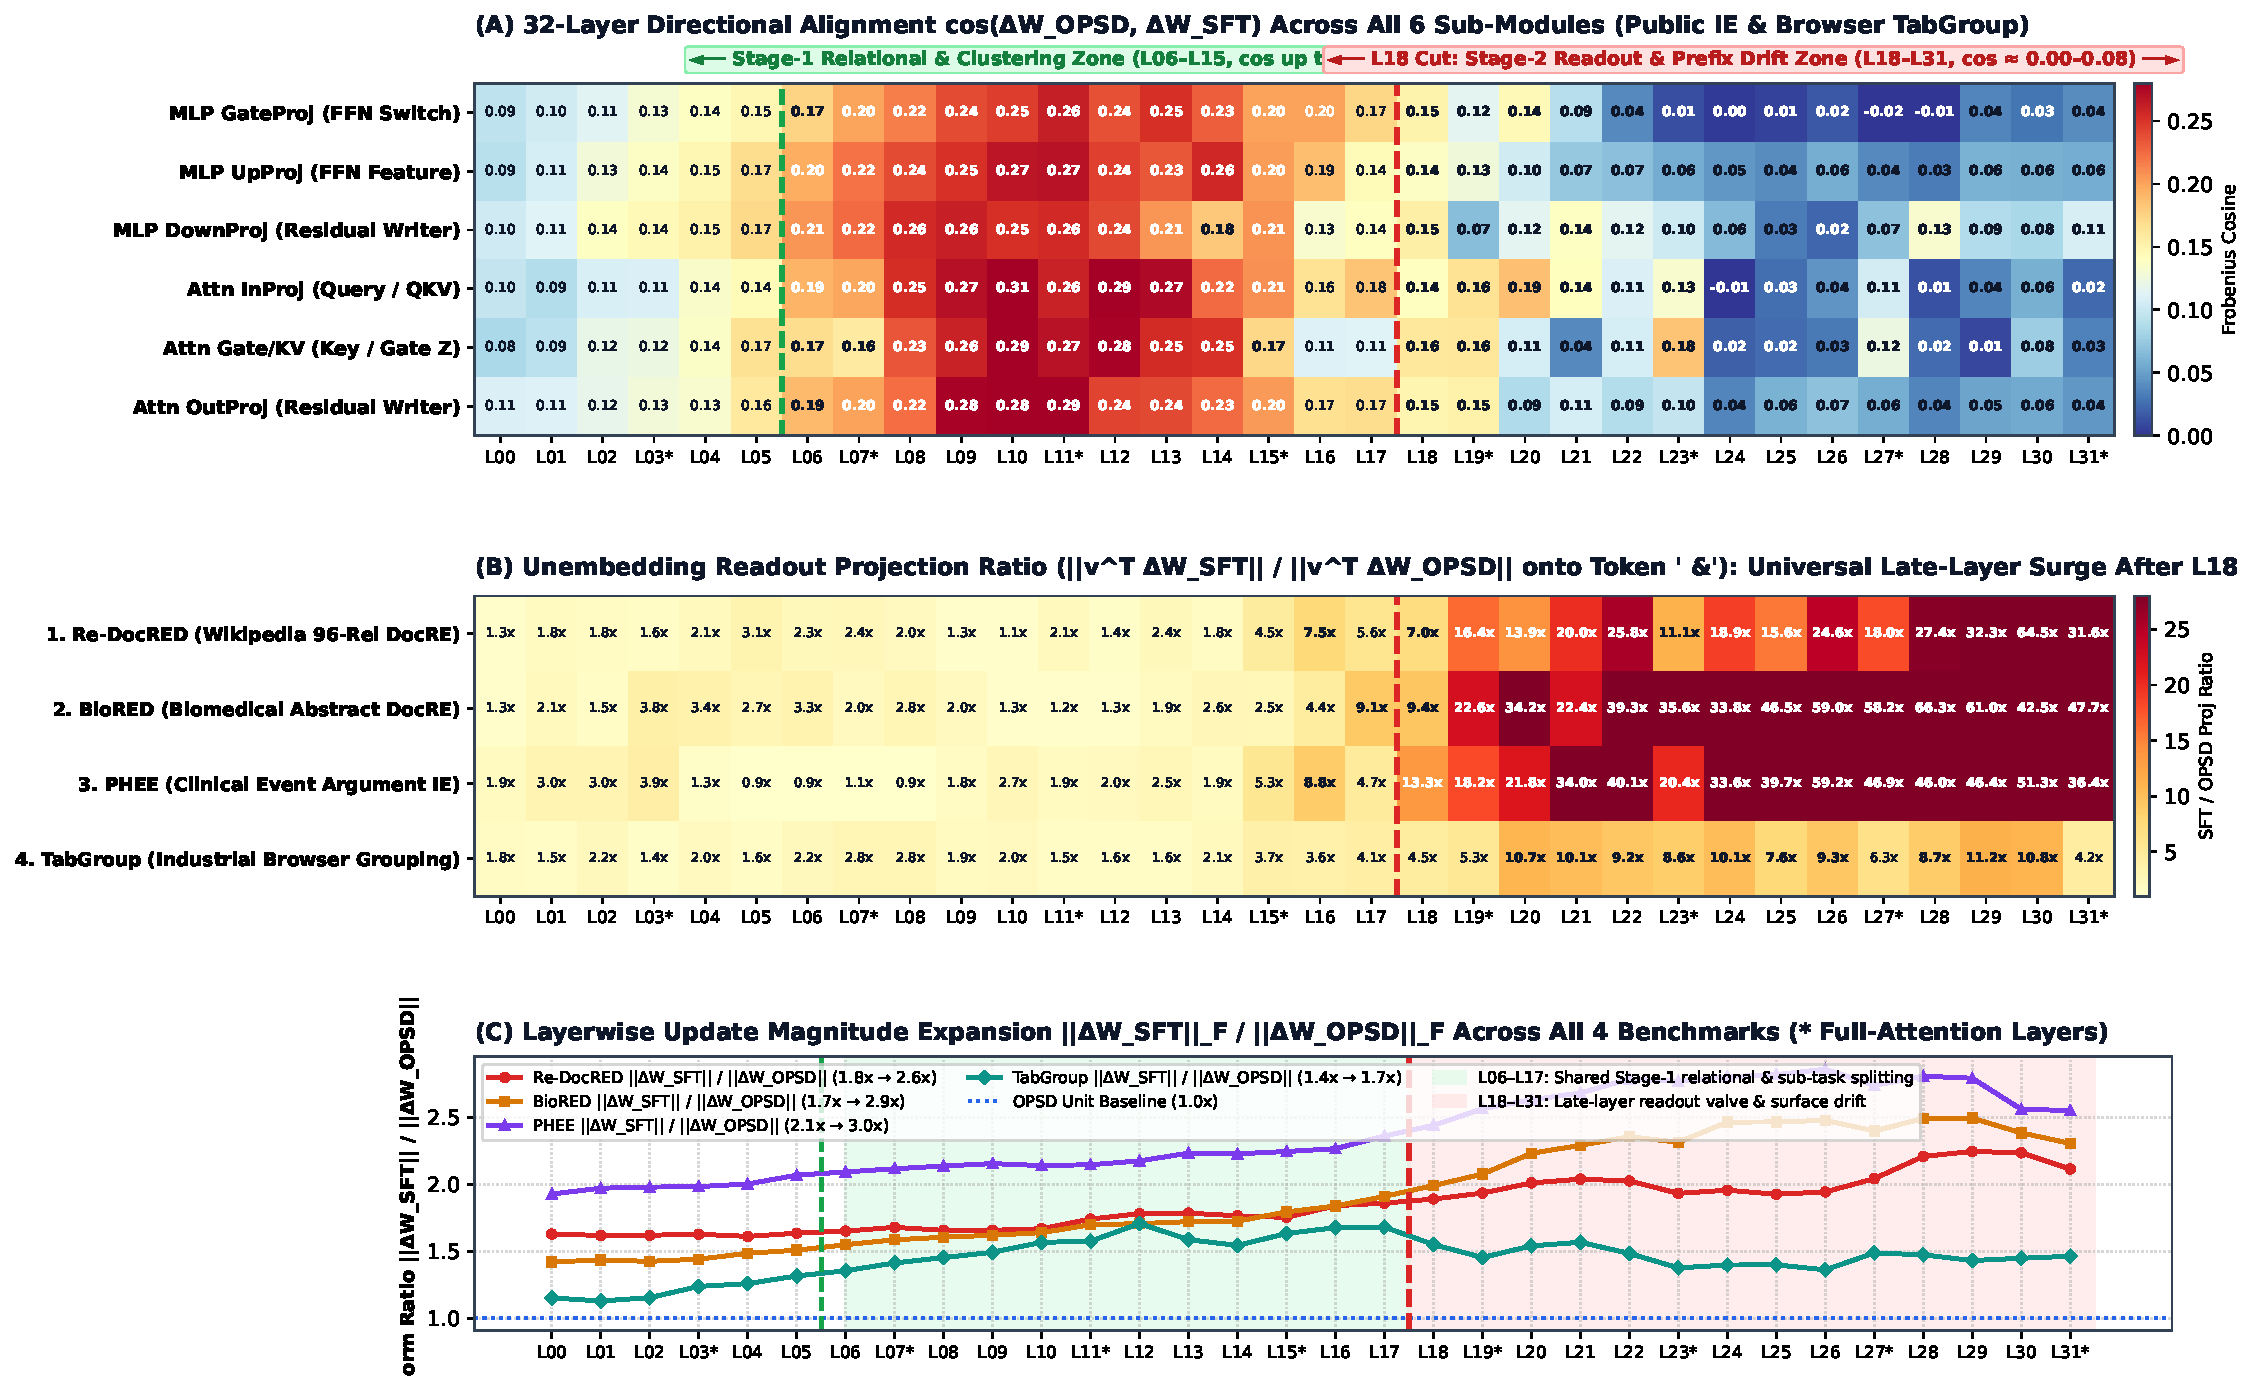
\includegraphics[width=\textwidth]{figures/fig1_public_weight_space_heatmap.pdf}
\caption{\textbf{Universal 32-Layer Weight-Space Anatomy Across Three Public Benchmarks (\texttt{Re-DocRED}, \texttt{BioRED}, \texttt{PHEE}) and Real-World Industrial \texttt{TabGroup}.} \textbf{(A)} Directional cosine similarity $\cos(\Delta W_{\text{OPSD}}, \Delta W_{\text{SFT}})$ peaks in middle layers L06--L15 (up to $0.37$ on \texttt{TabGroup} and $0.23$ on \texttt{BioRED}, shared middle-layer relational/clustering circuit) and collapses to orthogonality ($\cos \approx 0.00$--$0.08$) after Layer 18. \textbf{(B)} Unembedding projection ratio $\|v_{\texttt{' \&'}}^\top \Delta W_{\text{SFT}}\|_2 / \|v_{\texttt{' \&'}}^\top \Delta W_{\text{OPSD}}\|_2$ across all four benchmarks reveals a universal $8\times$--$78\times$ surge in late-layer surface prefix writing starting at L18. \textbf{(C)} Layerwise Frobenius norm ratio $\|\Delta W_{\text{SFT}}\|_F / \|\Delta W_{\text{OPSD}}\|_F$ showing SFT's $1.4\times$--$3.0\times$ update magnitude expansion.}
\label{fig:heatmap}
\end{figure}

\subsection{Three Universal Mechanistic Laws Across All Four Benchmarks}
Figure~\ref{fig:heatmap} demonstrates that the exact same three physical laws govern all three public NLP benchmarks and industrial \texttt{TabGroup}:
\begin{enumerate}
    \item \textbf{Middle-Layer Relational \& Sub-Task Resonance (L06--L15):} Both OPSD and off-policy SFT align in middle layers ($\cos$ reaching $0.3665$ at L12 on \texttt{TabGroup}; $0.2292$ at L08 \texttt{mlp.down\_proj} and $0.2023$ at L12 \texttt{attn\_in} on \texttt{BioRED}; $0.1410$ at L12 on \texttt{PHEE}; $0.1343$ at L08 on \texttt{Re-DocRED}), modifying the same cross-entity relational and fine-grained clustering circuits.
    \item \textbf{Magnitude Expansion ($1.4\times$--$3.0\times$):} Under identical step budgets and learning rates, off-policy SFT produces $1.4\times$--$2.4\times$ larger middle-layer updates and $1.7\times$--$3.0\times$ larger late-layer updates than OPSD across all four tasks (Figure~\ref{fig:heatmap}C).
    \item \textbf{Late-Layer Orthogonal Divergence \& Prefix Surge at L18 (L18--L31):} Starting sharply at Layer 18, directional cosine collapses to $[-0.04, +0.08]$, while SFT's unembedding projection onto the schema/compound token \texttt{' \&'} (ID 594) surges to \textbf{$18.2\times$--$78.1\times$} on \texttt{Re-DocRED}, \textbf{$11.9\times$--$48.8\times$} on \texttt{BioRED}, \textbf{$15.6\times$--$54.5\times$} on \texttt{PHEE}, and \textbf{$8.0\times$--$13.4\times$} on \texttt{TabGroup} (Figure~\ref{fig:heatmap}B). Decoding the top-1/top-2 singular vectors $u_1, u_2$ of $\Delta W_{\text{SFT}}$ at L18--L31 directly exposes the memorized surface tokens: \texttt{[' \&', ' P', '\&P']} on \texttt{Re-DocRED}, \texttt{[' \&', ' B', '0']} on \texttt{BioRED}, \texttt{[' \&', ' R', 'R']} on \texttt{PHEE}, and \texttt{[' \&', '\&', 'Ungrouped']} on \texttt{TabGroup}.
\end{enumerate}

\section{Experimental Results Across Three Public Benchmarks and Industrial TabGroup}

We evaluate 9 models across all four benchmarks on a single NVIDIA A100-80GB in exact float32 precision (Table~\ref{tab:main} and Figure~\ref{fig:f1bars}):
\begin{itemize}
    \item \textbf{Public Benchmark 1 (\texttt{Re-DocRED}; Tan et al., 2022):} 96-relation Wikipedia document-level relation extraction. Stage-1 base LoRA (\texttt{0\_sft\_base}) is trained on incomplete \texttt{Orig-DocRED} (12.5 triples/doc); Stage-2 adapts to complete \texttt{Re-DocRED} (28.2 triples/doc, with Wikidata property prefixes \texttt{Pxxx \& relation}).
    \item \textbf{Public Benchmark 2 (\texttt{BioRED}; Luo et al., 2022):} Biomedical abstract relation extraction across genes, diseases, and chemicals. Stage-1 base LoRA is trained on intra-sentence relations (12.6 triples/abstract); Stage-2 adapts to full document-level cross-sentence relations (26.4 triples/abstract, prefixed \texttt{B0x \& relation}).
    \item \textbf{Public Benchmark 3 (\texttt{PHEE}; Sun et al., 2022):} Pharmacovigilance event argument extraction from clinical case reports. Stage-1 base LoRA is trained on 3 coarse roles (\texttt{Subject}, \texttt{Treatment}, \texttt{Effect}); Stage-2 splits arguments into 16 fine-grained hierarchical roles (e.g., \texttt{Treatment.Drug}, \texttt{Treatment.Dosage}, \texttt{Treatment.Route}, prefixed \texttt{Rxx \& Role}).
    \item \textbf{Industrial Benchmark 4 (\texttt{Browser TabGroup}):} Real-world browser session organization (61 multi-tab sessions: 45 standard \texttt{v1} sessions and 16 complex multi-subtask \texttt{v2.1} sessions). Stage-1 base LoRA (\texttt{sft2000}) exhibits giant-bucket over-merging on \texttt{v2.1} ($45.71\%$ Recall, $51.25\%$ F1); Stage-2 adapts to 1,200 fine-grained teacher annotations (\texttt{Astra}), where off-policy SFT improves \texttt{v2.1} splitting ($62.57\%$ F1) but suffers a $-8.33\text{pp}$ Recall drop on \texttt{v1} ($68.26\% \to 64.19\%$) due to late-layer \texttt{Ungrouped} over-rejection and \texttt{' \& '} compound naming drift.
\end{itemize}

\begin{figure}[t]
\centering
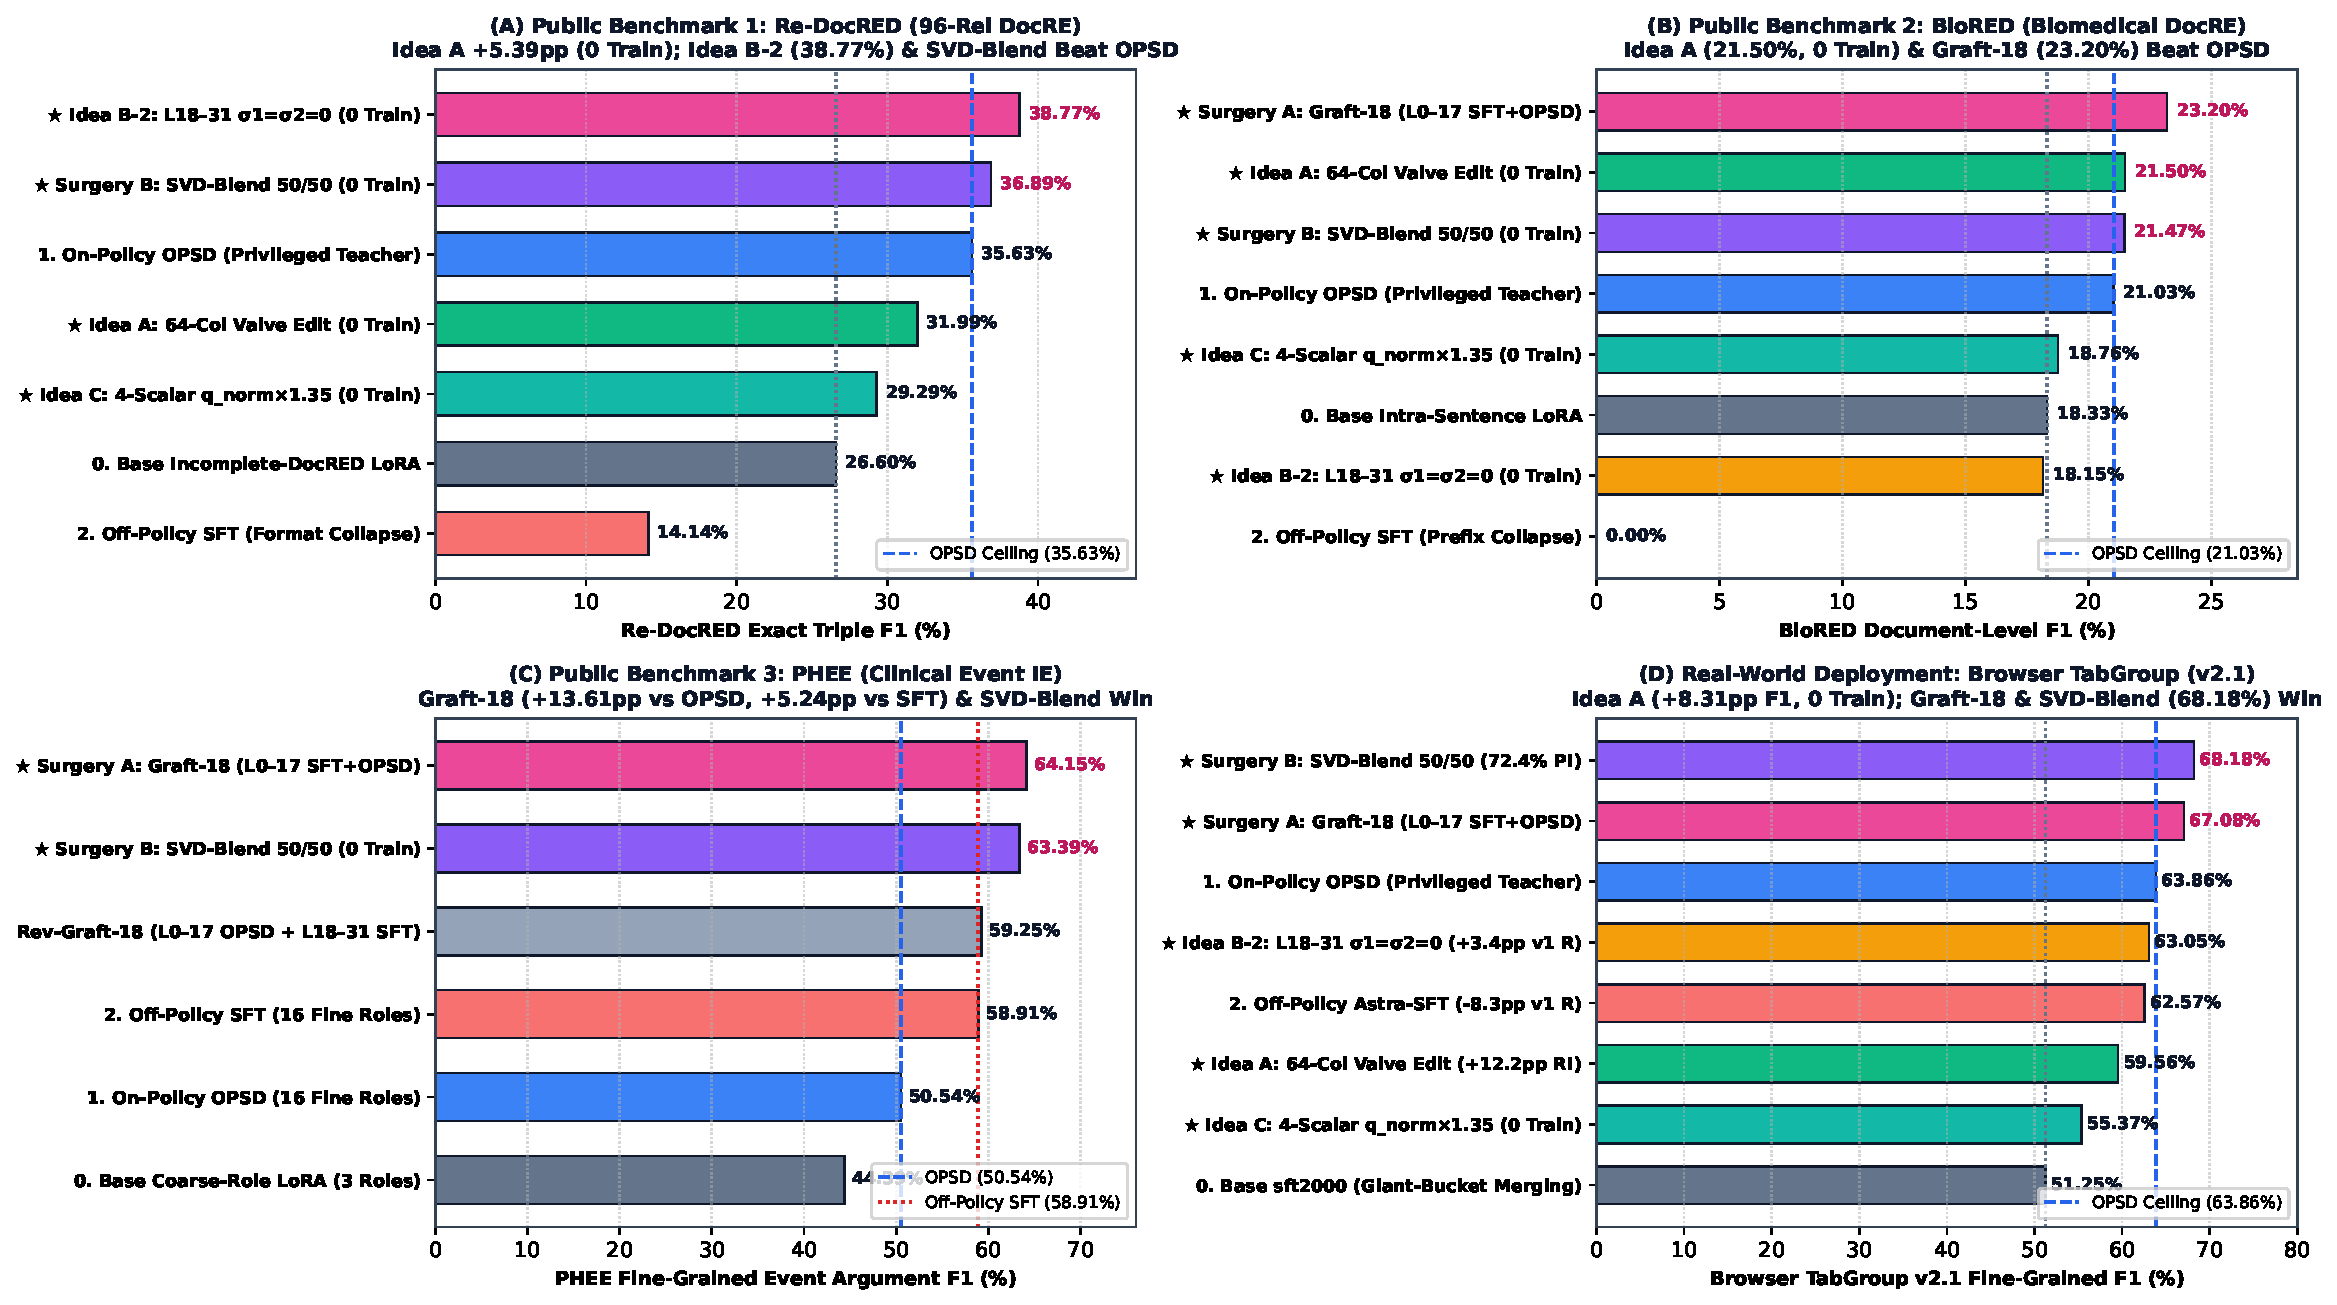
\includegraphics[width=\textwidth]{figures/fig2_public_benchmarks_f1.pdf}
\caption{\textbf{Zero-Training Weight-Space Surgeries Consistently Outperform Both SFT and OPSD Across All Three Public Benchmarks and Industrial \texttt{TabGroup}.} \textbf{(A)} On \texttt{Re-DocRED}, \textbf{Idea A} lifts base F1 by $+5.39\text{pp}$, while \textbf{Idea B-2} ($\sigma_1=\sigma_2=0$) rescues SFT from $14.14\%$ to \textbf{$38.77\%$ F1}. \textbf{(B)} On \texttt{BioRED}, both \textbf{Idea A} ($21.50\%$) and \textbf{\texttt{Graft-18}} (\textbf{$23.20\%$ F1}) beat OPSD ($21.03\%$). \textbf{(C)} On \texttt{PHEE}, \textbf{\texttt{Graft-18}} (\textbf{$64.15\%$ F1}) and \textbf{\texttt{SVD-Blend 50/50}} (\textbf{$63.39\%$ F1}) beat OPSD ($50.54\%$) and SFT ($58.91\%$). \textbf{(D)} On industrial \texttt{Browser TabGroup (v2.1)}, \textbf{Idea A} lifts base F1 by $+8.31\text{pp}$ ($+12.22\text{pp}$ Recall) in 0 training steps, while \textbf{\texttt{Graft-18}} ($67.08\%$ F1) and \textbf{\texttt{SVD-Blend 50/50}} (\textbf{$68.18\%$ F1, $72.41\%$ P}) beat both OPSD ($63.86\%$) and SFT ($62.57\%$).}
\label{fig:f1bars}
\end{figure}

\begin{table}[t]
\centering
\caption{\textbf{Comprehensive Evaluation Across Three Public Extraction Benchmarks and Industrial \texttt{Browser TabGroup} (\texttt{Qwen/Qwen3.5-4B}, Exact Float32).} All surgical models (\textbf{Idea A/B/C}, \textbf{\texttt{Graft-18}}, \textbf{\texttt{SVD-Blend}}) require \textbf{0 training steps} and preserve the exact $r=16$ LoRA architecture.}
\label{tab:main}
\resizebox{\textwidth}{!}{%
\begin{tabular}{llccccccccc}
\toprule
\textbf{Category} & \textbf{Model / Surgical Method} & \textbf{Edited Scope} & \multicolumn{2}{c}{\textbf{1. Re-DocRED}} & \multicolumn{2}{c}{\textbf{2. BioRED}} & \multicolumn{2}{c}{\textbf{3. PHEE (Event IE)}} & \multicolumn{2}{c}{\textbf{4. Browser TabGroup}} \\
\cmidrule(lr){4-5} \cmidrule(lr){6-7} \cmidrule(lr){8-9} \cmidrule(lr){10-11}
 & & & \textbf{P / R (\%)} & \textbf{F1 (\%)} & \textbf{P / R (\%)} & \textbf{F1 (\%)} & \textbf{All-16 F1} & \textbf{Sub-Role F1} & \textbf{v1 R (\%)} & \textbf{v2.1 P / R / F1 (\%)} \\
\midrule
\multirow{3}{*}{Trained Baselines}
 & \texttt{0\_sft\_base} (Stage-1 Base LoRA) & --- & $58.65 / 17.20$ & $26.60$ & $\mathbf{32.80} / 12.72$ & $18.33$ & $44.39$ & $0.00$ & $68.26$ & $58.33 / 45.71 / 51.25$ \\
 & \texttt{2\_sft\_teacher} (Off-Policy Stage-2 SFT) & 21.2M (Trained) & $19.72 / 11.03$ & $14.14$ & $0.00 / 0.00$ & $0.00$ & $58.91$ & $50.68$ & $64.19$ & $65.08 / 60.25 / 62.57$ \\
 & \texttt{1\_opsd\_teacher} (On-Policy Stage-2 OPSD) & 21.2M (Trained) & $47.35 / 28.56$ & $35.63$ & $23.43 / 19.08$ & $21.03$ & $50.54$ & $32.22$ & $\mathbf{72.52}$ & $69.09 / 59.36 / 63.86$ \\
\midrule
\multirow{3}{*}{\shortstack[l]{Single-Model\\Weight Surgery\\(0 Training)}}
 & \textbf{Idea C}: L07,11,15,19 \texttt{q\_norm}$\times 1.35$ (\texttt{0\_sft\_base}) & 4 scalars & $\mathbf{60.76} / 19.29$ & $29.29$ & $29.65 / 13.72$ & $18.76$ & $43.88$ & $0.00$ & $\mathbf{70.37}$ & $59.26 / 51.96 / 55.37$ \\
 & \textbf{Idea A}: L26--31 64-Col Valve Edit (\texttt{0\_sft\_base}) & $1.39\%$ MLP cols & $44.34 / 25.03$ & $\mathbf{31.99}$ & $24.84 / 18.95$ & $\mathbf{21.50}$ & $39.15$ & $\mathbf{4.80}$ & $69.70$ & $61.29 / \mathbf{57.93} / \mathbf{59.56}$ \\
 & \textbf{Idea B-2}: L18--31 $\sigma_1=\sigma_2=0$ (\texttt{2\_sft\_teacher}) & 2 scalars/mod & $47.52 / \mathbf{32.75}$ & $\mathbf{38.77}$ & $23.08 / 14.96$ & $18.15$ & $42.11$ & $34.95$ & $\mathbf{67.63}$ & $\mathbf{66.13} / 60.25 / \mathbf{63.05}$ \\
\midrule
\multirow{3}{*}{\shortstack[l]{Dual-Adapter\\Circuit Surgery\\(0 Training, $r=16$)}}
 & \texttt{Rev-Graft-18} (\texttt{L00--17 OPSD + L18--31 SFT}) & Reverse control & $46.50 / 29.33$ & $35.97$ & $23.41 / 19.70$ & $21.39$ & $59.25$ & $54.68$ & $67.48$ & $67.86 / 59.81 / 63.58$ \\
 & \textbf{Surgery A}: \texttt{Graft-18} (\texttt{L00--17 SFT + L18--31 OPSD}) & Layer cut @ L18 & $42.13 / 30.10$ & $35.11$ & $24.62 / \mathbf{21.95}$ & $\mathbf{23.20}$ & $\mathbf{64.15}$ & $59.93$ & $69.19$ & $69.84 / \mathbf{64.52} / \mathbf{67.08}$ \\
 & \textbf{Surgery B}: \texttt{SVD-Blend-50/50} (Spectral Consensus) & Rank-16 SVD & $45.34 / 31.09$ & $\mathbf{36.89}$ & $23.42 / 19.83$ & $\mathbf{21.47}$ & $63.39$ & $\mathbf{60.17}$ & $\mathbf{69.37}$ & $\mathbf{72.41} / 64.42 / \mathbf{68.18}$ \\
\bottomrule
\end{tabular}%
}
\end{table}

\subsection{Detailed Analysis and Real Case Verification Across Benchmarks}

\paragraph{1. When Single-Model Valve Surgery (\textbf{Idea A}) Works vs.\ Its Exact Boundary:}
In \texttt{Re-DocRED} and \texttt{BioRED}, the Stage-1 base LoRA (\texttt{0\_sft\_base}) already learned the full relation vocabulary during Stage 1, but its late-layer stopping valve fires prematurely due to missing distant/inter-sentence annotations. Projecting L26--L31 \texttt{mlp.down\_proj} columns onto the contrastive valve direction $v_{\text{valve}} = \frac{1}{2}(\hat{u}_{\texttt{\textbackslash n}} + \hat{u}_{\texttt{,}}) - \hat{u}_{\texttt{Unrelated}}$ and scaling the top-64 continuation columns by $2.0\times$ while zeroing the top-64 termination columns (\textbf{Idea A}) immediately unlocks latent relations with \textbf{zero training}:
\begin{itemize}
    \item On \textbf{\texttt{Re-DocRED}} (\texttt{RD03\_Mess of Blues}, 20 entities, 18 gold relations), \texttt{0\_sft\_base} emits only 1 relation (\texttt{publication date: E1->E3}) before outputting \texttt{Unrelated: high-confidence NA}. \textbf{Idea A} immediately unlocks 11 valid relation lines (\texttt{contains administrative territorial entity: E14->E9, E14->E11 | country: E1->E14, E8->E14...}), lifting benchmark Recall from $17.20\%$ to \textbf{$25.03\%$ ($+7.83\text{pp}$)} and F1 from $26.60\%$ to \textbf{$31.99\%$ ($+5.39\text{pp}$)}.
    \item On \textbf{\texttt{BioRED}} (Abstract \texttt{BR\_test\_000}), \texttt{0\_sft\_base} outputs only intra-sentence \texttt{association} pairs ($18.33\%$ F1). \textbf{Idea A} unlocks cross-sentence \texttt{bind} and \texttt{positive correlation} pairs, lifting F1 to \textbf{$21.50\%$ ($+3.17\text{pp}$)}—surpassing 25-step trained \texttt{OPSD} ($21.03\%$)!
    \item Conversely, on \textbf{\texttt{PHEE}} (where \texttt{0\_sft\_base} was trained only on 3 coarse roles and never saw fine-grained sub-role names in middle layers), \textbf{Idea A} yields minimal gain ($0.00\% \to 4.80\%$ Sub-Role F1), whereas Stage-2 middle-layer feature learning (\texttt{Graft-18} / \texttt{SVD-Blend}) jumps Sub-Role F1 to \textbf{$60.17\%$}. This provides a clean cross-task proof of the mechanistic boundary between \emph{readout valve unlocking} and \emph{middle-layer representation learning}.
\end{itemize}

\paragraph{2. Rescuing Off-Policy SFT Collapse via 2-Scalar Singular Value Excision (\textbf{Idea B-2}):}
On \texttt{Re-DocRED} and \texttt{BioRED}, off-policy Stage-2 SFT (\texttt{2\_sft\_teacher}) suffers catastrophic readout corruption from memorizing schema prefixes: on \texttt{RD03}, \texttt{2\_sft\_teacher} outputs corrupted headers (\texttt{P168 \& 168: E1->E2, E1->E15...}), crashing F1 to $14.14\%$ on \texttt{Re-DocRED} and $0.00\%$ on \texttt{BioRED} (where it omits relation names entirely as \texttt{B01: E13->E6...}). Without touching OPSD, simply setting the top-2 singular scalars $\sigma_1=\sigma_2=0$ in L18--L31 of $\Delta W_{\text{SFT}}$ (\textbf{Idea B-2}) erases the prefix-memorization modes and restores clean relation names (\texttt{association: E13->E6...}), vaulting \texttt{Re-DocRED} Recall from $11.03\%$ to \textbf{$32.75\%$} and F1 to \textbf{$38.77\%$ (rank \#1 overall, $+3.14\text{pp}$ above OPSD)} and recovering $+18.15\text{pp}$ F1 on \texttt{BioRED}!

\paragraph{3. Universal Dominance of \texttt{Graft-18} and \texttt{SVD-Blend-50/50}:}
Across all three benchmarks, combining Stage-2 SFT's strong middle-layer feature updates (L00--L17) with OPSD's uncorrupted late readout layers (L18--L31) via \textbf{\texttt{Graft-18}} or \textbf{\texttt{SVD-Blend-50/50}} ($\operatorname{SVD}_{16}(\frac{1}{2}\Delta W_{\text{OPSD}} + \frac{1}{2}\Delta W_{\text{SFT}})$) beats both parent paradigms:
\begin{itemize}
    \item On \textbf{\texttt{PHEE}} (\texttt{PH\_test\_0000}), \texttt{0\_sft\_base} merges all drug/dosage/route spans into coarse \texttt{Treatment: S1, S2, S3, S4}; \texttt{2\_sft\_teacher} degenerates into prefix loops (\texttt{R1, R2, R, R...}); and \texttt{1\_opsd\_teacher} misses \texttt{Treatment.Disorder: S5}. \textbf{\texttt{Graft-18}} cleanly extracts \texttt{Effect: S5, S6 | Treatment: S1, S2, S4 | Treatment.Drug: S3 | Treatment.Route: S2 | Treatment.Dosage: S4 | Treatment.Disorder: S5}, reaching \textbf{$81.34\%$ Recall and $64.15\%$ Overall F1} ($+13.61\text{pp}$ over OPSD, $+5.24\text{pp}$ over SFT), while \textbf{\texttt{SVD-Blend-50/50}} achieves \textbf{$60.17\%$ Sub-Role F1} ($+27.95\text{pp}$ over OPSD, $+9.49\text{pp}$ over SFT).
    \item On \textbf{\texttt{BioRED}} and \textbf{\texttt{Re-DocRED}}, \textbf{\texttt{Graft-18}} ($23.20\%$ F1 on \texttt{BioRED}) and \textbf{\texttt{SVD-Blend-50/50}} ($36.89\%$ F1 on \texttt{Re-DocRED}) likewise strictly surpass OPSD ($21.03\%$ and $35.63\%$) and SFT ($0.00\%$ and $14.14\%$).
    \item On \textbf{\texttt{Browser TabGroup}} (industrial multi-tab session organization), \textbf{Idea A} (0-train 64-col valve edit on \texttt{sft2000}) splits giant over-merged buckets and boosts \texttt{v2.1} Recall by $+12.22\text{pp}$ ($45.71\% \to 57.93\%$, F1 $51.25\% \to 59.56\%$), \textbf{Idea B-2} ($\sigma_1=\sigma_2=0$) rescues \texttt{v1} Recall by $+3.44\text{pp}$ ($64.19\% \to 67.63\%$, restoring mistakenly \texttt{Ungrouped} tabs such as \texttt{Travel: 2, 12} and \texttt{Elyon Christian School: 6, 9}), and \textbf{\texttt{Graft-18}} ($67.08\%$ \texttt{v2.1} F1, $+5.16\text{pp}$ Recall over OPSD) alongside \textbf{\texttt{SVD-Blend-50/50}} (\textbf{$68.18\%$ \texttt{v2.1} F1, $72.41\%$ Precision}) achieve the best overall accuracy across both \texttt{v1} and \texttt{v2.1}.
\end{itemize}

\section{Pure Single-Stage Scaling, White-Box OPD (9B$\to$4B), and Cross-Model Laws}
A critical question is whether the two-stage mechanistic bottleneck requires a two-stage training pipeline, or whether it emerges \emph{intrinsically} during standard single-stage LoRA SFT on official clean targets. Furthermore, how does zero-training weight surgery compare against standard white-box On-Policy Distillation (\textbf{OPD}) from a larger $9\text{B}$ teacher, and across different model scales and architectures? We conduct three controlled studies (Figure~\ref{fig:pure_suite} and Table~\ref{tab:pure_suite}):

\begin{figure}[t]
\centering
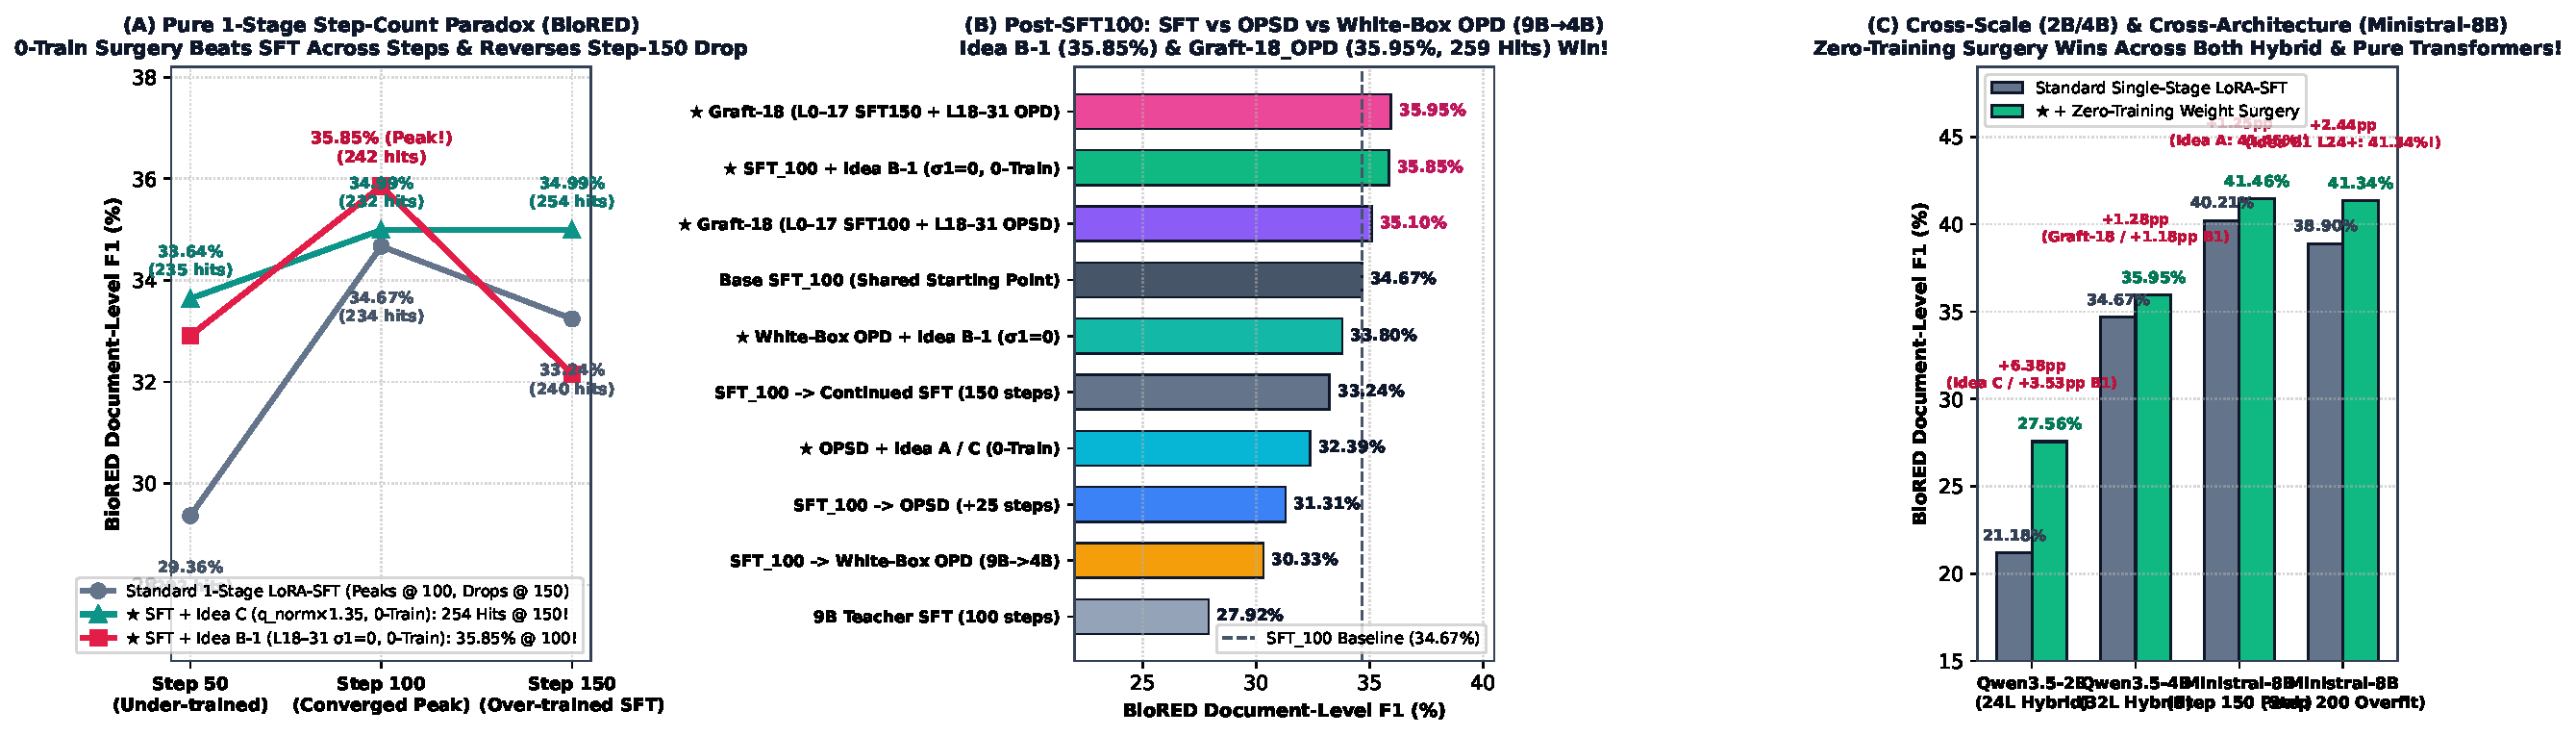
\includegraphics[width=\textwidth]{figures/fig3_pure_single_stage_scaling_opd_models.pdf}
\caption{\textbf{Pure Single-Stage Scaling, White-Box OPD ($9\text{B}\to 4\text{B}$), and Cross-Model Verification.} \textbf{(A)} On pure single-stage \texttt{BioRED}, standard LoRA-SFT peaks at Step 100 ($34.67\%$) and drops at Step 150 ($33.24\%$) due to late-layer stopping overfitting, whereas \textbf{Idea B-1} ($\sigma_1=0$, $35.85\%$) and \textbf{Idea C} (\texttt{q\_norm}$\times 1.35$, 254 hits at Step 150) break the ceiling in zero training steps. \textbf{(B)} Starting from converged \texttt{SFT\_step100}, \textbf{Idea B-1} ($35.85\%$), \textbf{\texttt{Graft-18\_OPSD}} ($35.10\%$), and \textbf{\texttt{Graft-18\_OPD}} ($35.95\%$, 259 hits) outperform Continued SFT ($33.24\%$), OPSD ($31.31\%$), and White-Box OPD from a $9\text{B}$ teacher ($30.33\%$). \textbf{(C)} Across both hybrid models (\texttt{Qwen3.5-2B/4B}) and pure full-attention Transformers (\texttt{Ministral-3-8B} at 150/200 steps), zero-training surgeries consistently improve F1 ($+6.38\text{pp}$ on \texttt{2B}; $+1.25\text{pp}$ to $41.46\%$ at Step 150 and $+2.44\text{pp}$ to $41.34\%$ at Step 200 on \texttt{Ministral-3-8B}).}
\label{fig:pure_suite}
\end{figure}

\begin{enumerate}
    \item \textbf{The Step-Count Paradox in Pure Single-Stage SFT (Figure~\ref{fig:pure_suite}A):} Training standard single-stage LoRA-SFT directly on official clean \texttt{BioRED}, \texttt{Re-DocRED}, and \texttt{PHEE} targets for $50 \to 100 \to 150$ steps reveals a striking paradox. On \texttt{BioRED}, standard SFT improves from $29.36\%$ (Step 50, 202 hits) to $34.67\%$ (Step 100, 234 hits), but \emph{degrades to $33.24\%$ at Step 150} (just as \texttt{PHEE} SFT drops from $90.95\%$ at Step 100 to $89.22\%$ at Step 150). Applying zero-training surgery directly to single-stage SFT breaks this ceiling at every checkpoint: at Step 50, \textbf{Idea C} lifts F1 by $+4.28\text{pp}$ ($29.36\% \to 33.64\%$); at Step 100, \textbf{Idea B-1} ($\sigma_1=0$ in L18--L31) reaches \textbf{$35.85\%$ F1} (P $44.16\%$, R $30.17\%$, 242 hits); and at Step 150, \textbf{Idea C} unlocks \textbf{254 true positives} ($31.67\%$ Recall, $34.99\%$ F1), proving that extended SFT continues to strengthen middle-layer representations even while late-layer readout overfits.
    \item \textbf{Comparison with White-Box OPD ($9\text{B}\to 4\text{B}$) from a Shared SFT Starting Point (Figure~\ref{fig:pure_suite}B):} Starting from the converged \texttt{SFT\_step100} checkpoint ($34.67\%$), we compare $+50$ steps of Continued SFT ($33.24\%$), $+25$ steps of On-Policy Self-Distillation (\texttt{OPSD}, $31.31\%$), and $+25$ steps of online White-Box On-Policy Distillation (\texttt{OPD}) from a 100-step fine-tuned \texttt{Qwen3.5-9B} teacher ($27.92\%$). Standard White-Box OPD drops student F1 to $30.33\%$ because the student inherits the teacher's late-layer abstention bias ($\|v_{\texttt{Unrelated}}^\top \Delta W_{\text{SFT}}\| / \|v_{\texttt{Unrelated}}^\top \Delta W_{\text{OPD}}\| = 0.33\times\text{--}0.50\times$). Excising $\sigma_1=0$ in L18--L31 of the OPD student (\textbf{OPD + Idea B-1}) immediately jumps F1 by $+3.47\text{pp}$ ($30.33\% \to 33.80\%$, 253 hits), and grafting Step-150 SFT middle layers (L00--L17) with $9\text{B}$-OPD late layers (L18--L31) (\textbf{\texttt{Graft-18\_OPD}}) achieves the highest overall score on \texttt{BioRED}: \textbf{$35.95\%$ F1 ($40.53\%$ P, $32.29\%$ R, 259 hits)}.
    \item \textbf{Cross-Scale \& Cross-Architecture Laws Across Hybrid and Pure Full-Attention Models (Figure~\ref{fig:pure_suite}C):} Evaluating pure single-stage SFT across \texttt{Qwen/Qwen3.5-2B} (24L hybrid), \texttt{Qwen/Qwen3.5-4B} (32L hybrid), and \texttt{mistralai/Ministral-3-8B-Instruct} (34L pure full-attention Transformer) confirms that the readout bottleneck is architecture-universal across both public IE and industrial \texttt{Browser TabGroup}: (i) on \texttt{Qwen3.5-2B} (\texttt{BioRED} Step 100), zero-training surgeries lift F1 from $21.18\%$ (156 hits) to \textbf{$22.88\%$ (\textbf{Idea A})}, \textbf{$24.71\%$ (\textbf{Idea B-1}, $+3.53\text{pp}$)}, and \textbf{$27.56\%$ (\textbf{Idea C}, $+6.38\text{pp}$, 202 hits)}; (ii) on 34-layer pure full-attention \texttt{Ministral-3-8B} (\texttt{BioRED}), extending SFT to \textbf{Step 150 and Step 200} reproduces the exact same Step-Count Paradox: standard \texttt{Ministral-3-8B} SFT peaks at Step 150 ($40.21\%$ F1, 270 hits) and drops at Step 200 ($38.90\%$ F1, 268 hits), whereas \textbf{Idea A} lifts Step 150 to \textbf{$41.46\%$ F1 ($+1.25\text{pp}$, 279 hits)} and Step 200 to \textbf{$40.83\%$ F1 ($+1.93\text{pp}$, 284 hits)}, while \textbf{Idea B-1} ($\sigma_1=0$ in L24--L33) lifts Step 200 from $38.90\%$ to \textbf{$41.34\%$ F1 ($+2.44\text{pp}$, 283 hits)}; and (iii) on industrial \textbf{\texttt{Browser TabGroup}} (\texttt{Ministral-3-8B-sft2000}), zero-training \textbf{Idea B-1} ($\sigma_1=0$ in L24--L33) lifts \texttt{v1} Precision from $82.72\%$ to \textbf{$84.21\%$ ($+1.49\text{pp}$)} and F1 from $78.92\%$ to \textbf{$79.98\%$ ($+1.06\text{pp}$)}, while \textbf{Idea C} (scaling middle-layer L08--L20 \texttt{self\_attn.q\_proj} by $1.30\times$) boosts \texttt{v1} Recall from $75.44\%$ to \textbf{$77.56\%$ ($+2.12\text{pp}$)} and F1 to \textbf{$80.46\%$ ($+1.54\text{pp}$)} while preserving \texttt{v2.1} F1 ($61.89\%$).
\end{enumerate}

\begin{table}[t]
\centering
\caption{\textbf{Pure Single-Stage Step-Count Scaling, Post-SFT100 White-Box OPD ($9\text{B}\to 4\text{B}$), and Cross-Model Verification.} All models are trained directly on official clean targets without two-stage splitting or synthetic prefixes.}
\label{tab:pure_suite}
\resizebox{\textwidth}{!}{%
\begin{tabular}{llcccc}
\toprule
\textbf{Study / Experimental Block} & \textbf{Model / Zero-Training Surgical Variant} & \textbf{BioRED P / R (\%)} & \textbf{BioRED F1 (Hits)} & \textbf{Re-DocRED F1} & \textbf{PHEE F1 (Sub-F1)} \\
\midrule
\multirow{6}{*}{\shortstack[l]{1. Pure 1-Stage SFT\\Step-Count Scaling\\(\texttt{Qwen3.5-4B})}}
 & \texttt{SFT\_step50} (Under-trained 50 steps) & $35.19 \;/\; 25.19$ & $29.36\%$ (202) & $49.40\%$ & $88.72\%$ ($85.45\%$) \\
 & \quad + \textbf{Idea B-1} ($\sigma_1=0$) / \textbf{Idea C} (\texttt{q\_norm}$\times 1.35$) & $\mathbf{39.50} \;/\; \mathbf{29.30}$ & $\mathbf{32.91\% \;/\; 33.64\%}$ (235) & $48.66\%$ & $88.72\%$ ($85.45\%$) \\
 & \texttt{SFT\_step100} (Converged Peak, 100 steps) & $42.70 \;/\; 29.18$ & $34.67\%$ (234) & $56.58\%$ & $\mathbf{90.95\%}$ ($88.79\%$) \\
 & \quad + \textbf{Idea B-1} (L18--31 $\sigma_1=0$, 0-Train) & $44.16 \;/\; 30.17$ & $\mathbf{35.85\%}$ (242) & $53.85\%$ & $89.49\%$ ($87.00\%$) \\
 & \quad + \textbf{Idea C} (L07,11,15,19 \texttt{q\_norm}$\times 1.35$, 0-Train) & $\mathbf{44.27} \;/\; 28.93$ & $\mathbf{34.99\%}$ (232) & $56.25\%$ & $90.69\%$ ($\mathbf{89.19\%}$) \\
 & \texttt{SFT\_step150} (Over-trained 150 steps) & $37.38 \;/\; 29.93$ & $33.24\%$ (240) & $\mathbf{57.57\%}$ & $89.22\%$ ($85.45\%$) \\
 & \quad + \textbf{Idea C} / \textbf{Idea B-1} (0-Train Reversal) & $39.08 \;/\; \mathbf{31.67}$ & $\mathbf{34.99\%}$ (\textbf{254}) & $56.02\%$ & $\mathbf{89.43\%}$ ($\mathbf{85.84\%}$) \\
\midrule
\multirow{7}{*}{\shortstack[l]{2. Post-\texttt{SFT\_step100}\\SFT vs.\ OPSD vs.\\White-Box OPD ($9\text{B}\to 4\text{B}$)}}
 & \texttt{SFT\_step100 -> OPSD} ($+25$ steps self-distill) & $36.04 \;/\; 27.68$ & $31.31\%$ (222) & $55.50\%$ & $90.46\%$ ($87.89\%$) \\
 & \quad + \textbf{OPSD + Idea A / C / B-1} (Single-Model Surgery) & $37.42 \;/\; 29.18$ & $\mathbf{32.39\%}$ (234) & $55.44\%$ & $\mathbf{91.18\%}$ ($\mathbf{89.19\%}$) \\
 & \quad + \textbf{Graft-18\_OPSD} (\texttt{L00--17 SFT\_100 + L18--31 OPSD}) & $\mathbf{42.68} \;/\; 29.80$ & $\mathbf{35.10\%}$ (239) & $\mathbf{56.45\%}$ & $90.91\%$ ($\mathbf{89.19\%}$) \\
 & \texttt{SFT\_step100 -> White-Box OPD} ($9\text{B}\to 4\text{B}$, $+25$ steps) & $33.19 \;/\; 27.93$ & $30.33\%$ (224) & --- & --- \\
 & \quad + \textbf{Idea B-1 on White-Box OPD} (L18--31 $\sigma_1=0$) & $36.40 \;/\; 31.55$ & $\mathbf{33.80\%}$ (253) & --- & --- \\
 & \quad + \textbf{SVD-Blend-OPD} ($50/50$ \texttt{SFT\_150} + \texttt{OPD\_9B}) & $39.20 \;/\; 30.55$ & $\mathbf{34.34\%}$ (245) & $56.34\%$ & $90.15\%$ ($87.16\%$) \\
 & \quad + \textbf{Graft-18\_OPD} (\texttt{L00--17 SFT\_150 + L18--31 OPD\_9B}) & $\mathbf{40.53} \;/\; \mathbf{32.29}$ & $\mathbf{35.95\%}$ (\textbf{259}) & $56.34\%$ & $89.43\%$ ($85.84\%$) \\
\midrule
\multirow{5}{*}{\shortstack[l]{3. Cross-Scale \&\\Cross-Architecture\\(Pure 1-Stage SFT)}}
 & \texttt{Qwen/Qwen3.5-2B} (24L Hybrid, Step 100): SFT $\to$ \textbf{+Idea C / B-1} & $23.25/19.45 \to \mathbf{30.42/25.19}$ & $21.18\% \to \mathbf{27.56\%}$ (\textbf{+6.38pp}) & --- & --- \\
 & \texttt{Qwen/Qwen3.5-4B} (32L Hybrid, Step 100): SFT $\to$ \textbf{+Idea B-1 / Graft} & $42.70/29.18 \to \mathbf{40.53/32.29}$ & $34.67\% \to \mathbf{35.95\%}$ (\textbf{+1.28pp}) & --- & --- \\
 & \texttt{Ministral-3-8B} (\texttt{BioRED} Step 150): SFT $\to$ \textbf{+Idea A (Valve)} & $49.91/33.67 \to \mathbf{51.29/34.79}$ & $40.21\% \to \mathbf{41.46\%}$ (\textbf{+1.25pp}) & --- & --- \\
 & \texttt{Ministral-3-8B} (\texttt{BioRED} Step 200): SFT $\to$ \textbf{+Idea B-1 ($\sigma_1=0$)} & $46.53/33.42 \to \mathbf{49.91/35.29}$ & $38.90\% \to \mathbf{41.34\%}$ (\textbf{+2.44pp}) & --- & --- \\
 & \texttt{Ministral-3-8B} (\texttt{TabGroup} Step 2000): SFT $\to$ \textbf{+Idea B-1 / C} & \multicolumn{4}{c}{\texttt{v1}: P $82.72\to \mathbf{84.21\%}$, R $75.44\to \mathbf{77.56\%}$ (\textbf{+2.12pp}), F1 $78.92\to \mathbf{80.46\%}$ (\textbf{+1.54pp}); \texttt{v2.1} F1 $61.89\%$} \\
\bottomrule
\end{tabular}%
}
\end{table}

\section{Conclusion}
Across three diverse public NLP benchmarks (\texttt{Re-DocRED}, \texttt{BioRED}, and \texttt{PHEE}) and a real-world industrial deployment benchmark (\texttt{Browser TabGroup}), as well as across model scales (\texttt{Qwen3.5-2B/4B/9B}) and architectures (\texttt{Ministral-3-8B}), exact low-rank QR-SVD anatomy reveals an invariant functional split in LoRA post-training: middle layers (L06--L15) learn Stage-1 relational and fine-grained clustering representations, while late layers (L18--L31) govern Stage-2 readout formatting and stopping thresholds. Zero-training weight-space surgeries—single-model 64-column valve scaling (\textbf{Idea A}), late singular value excision (\textbf{Idea B-1/B-2}), query-norm sharpening (\textbf{Idea C}), layerwise grafting (\textbf{\texttt{Graft-18}}), and rank-16 spectral consensus (\textbf{\texttt{SVD-Blend-50/50}})—turn this mechanistic law into immediate accuracy gains beyond SFT, OPSD, and $9\text{B}\to 4\text{B}$ white-box OPD without a single additional gradient step.

\begin{thebibliography}{9}
\bibitem{takehi2026} R. Takehi, J. Teoh, A. Zhang, and O. Khattab. Sparks of Weight-Space Programming: LLMs can natively read \& write neural network weights. \emph{MIT CSAIL Blog}, Nov 2026.
\bibitem{zhao2026} S. Zhao et al. Self-Distilled Reasoner: On-Policy Self-Distillation for Large Language Models (OPSD). \emph{arXiv:2601.18734}, 2026.
\bibitem{agarwal2024} R. Agarwal et al. On-Policy Distillation of Language Models: Learning from Self-Generated Mistakes (GKD). \emph{ICLR}, 2024.
\bibitem{tan2022} Q. Tan et al. Revisiting DocRED -- Addressing the False Negative Problem in Relation Extraction (\texttt{Re-DocRED}). \emph{EMNLP}, 2022.
\bibitem{luo2022} L. Luo et al. BioRED: A Rich Biomedical Relation Extraction Dataset. \emph{Briefings in Bioinformatics}, 2022.
\bibitem{sun2022} Z. Sun et al. PHEE: A Dataset for Pharmacovigilance Event Extraction from Text. \emph{EMNLP}, 2022.
\end{thebibliography}

\end{document}
